\documentclass[10pt]{beamer}

\usetheme[progressbar=frametitle]{metropolis}
\usepackage{appendixnumberbeamer}

\usepackage[ngerman]{babel}
\usepackage[latin1]{inputenc}

\usepackage{booktabs}
\usepackage[scale=2]{ccicons}

\usepackage{pgfplots}
\usepgfplotslibrary{dateplot}

\usepackage{xspace}
\newcommand{\themename}{\textbf{\textsc{metropolis}}\xspace}

\title{R�ckgekoppelte neuronale Netze}
\subtitle{Eine Einf�hrung}
% \date{\today}
\date{}
\author{Konstantin Tieber}
\institute{webfactory GmbH}
% \titlegraphic{\hfill\includegraphics[height=1.5cm]{logo.pdf}}

\begin{document}

\maketitle

%\begin{frame}{Inhalt}
%  \setbeamertemplate{section in toc}[sections numbered]
%  \tableofcontents[hideallsubsections]
%\end{frame}

%\section{Einf�hrung in r�ckgekoppelte Netze}

\begin{frame}{Warum r�ckgekoppelte neuronale Netze?}
	\begin{itemize}
		\item eignet sich sehr gut zur Verarbeitung von Daten, die eine Sequenz darstellen
		\item Anwendungsbereiche\begin{itemize}
			\item Sprachverarbeitung
			\item Audioverarbeitung
			\item Videoverarbeitung
			\item Sprachmodellierung
		\end{itemize}
		%HIER DEMO Sprachmodellierung
	\end{itemize}
\end{frame}

\begin{frame}{R�ckgekoppelte Netze}
	\begin{figure}
		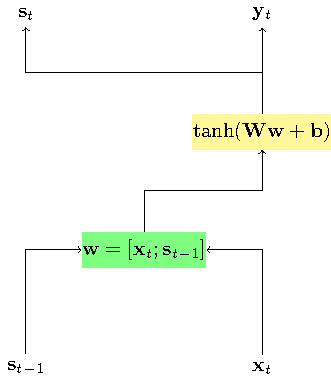
\includegraphics[scale=1]{../bilder_intro/recurrent_cell.pdf}
		\caption{Einfache r�ckgekoppelte Zelle.}
		%vanishing gradient problem
		%simple r�ckgekoppelte neuronale Netze funktionieren deswegen nicht
	\end{figure}
\end{frame}

\begin{frame}{Probleme}
	\begin{itemize}
		\item verschwindender Gradient % unbesiegbar?
		\item explodierender Gradient % clipping Funktion, um gro�e Zahlen abzurasieren
	\end{itemize}
\end{frame}

\begin{frame}{L�sung}
	\begin{figure}
		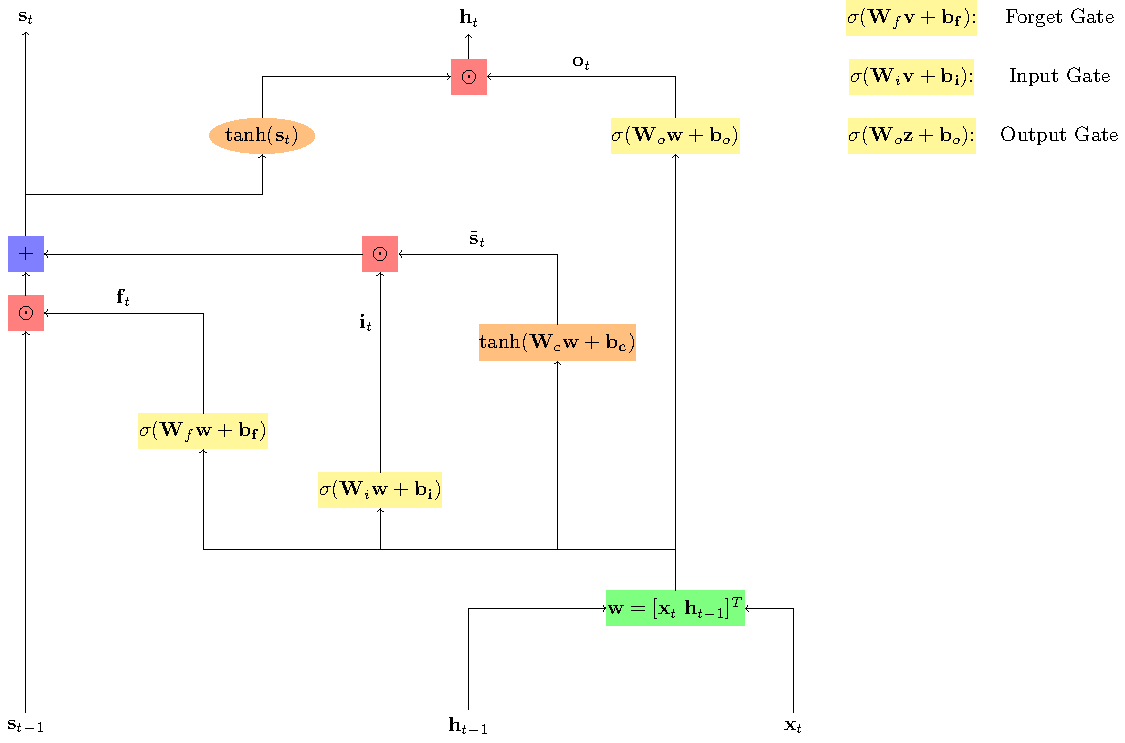
\includegraphics[scale=0.5]{../bilder_intro/nop_lstm.pdf}
		\caption{Schematische Darstellung einer Long Short Term Memory Zelle.}
	\end{figure}
\end{frame}

\begin{frame}{Problem}
	\begin{itemize}
		\item Wir bestimmen, was vergessen werden soll, ohne den Inhalt des Speichers zu kennen.
	\end{itemize}
\end{frame}

\begin{frame}{L�sung}
	\begin{figure}
		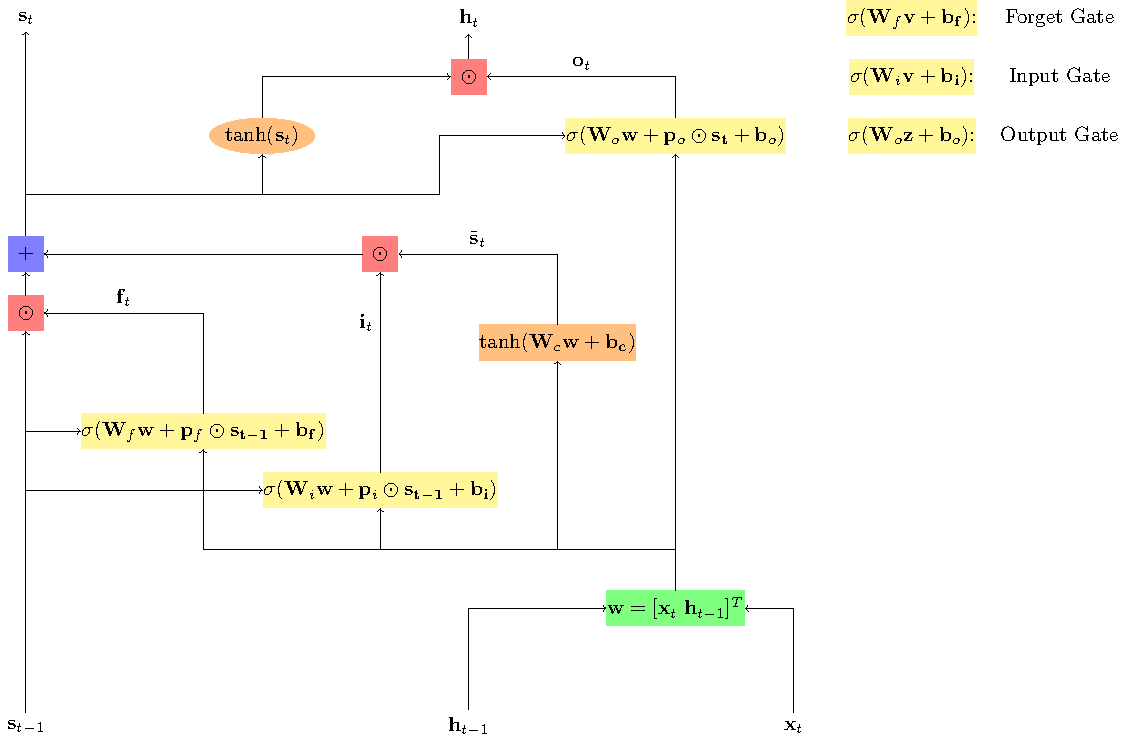
\includegraphics[scale=0.5]{../bilder_intro/lstm.pdf}
		\caption{Schematische Darstellung einer Long Short Term Memory Zelle mit Kuckl�chern.}
	\end{figure}
\end{frame}

\begin{frame}{Zusammenfassung}
	\begin{itemize}
		\item tbd
	\end{itemize}
\end{frame}

\end{document}
